% \usepackage{crimson} % Crimson Font
%\usepackage{CormorantGaramond} % Cormorant Garamond
%\usepackage[type1]{plex-serif} 
%\usepackage[type1, sb]{plex-serif} % semibold option for lighter bold fonts
%\usepackage[type1, m]{plex-serif} % medium option for lighter bold fonts
%\usepackage[type1, tx]{plex-serif} % text option for lighter bold fonts
%\usepackage[type1, l]{plex-serif} % light option for lighter regular fonts
%\usepackage[type1, el]{plex-serif} % extra light option for lighter regular fonts
%\usepackage[type1, t]{plex-serif} % thin option for lighter regular fonts
%\usepackage[type1, txmd]{plex-serif} % slightly heavier regular fonts
%\usepackage[type1, textmd]{plex-serif} % slightly heavier regular fonts
%\usepackage[tx]{plex-sans} 
% \usepackage[sfdefault]{plex-sans}
%\usepackage[sfdefault, sb]{plex-sans} % semibold option for lighter bold fonts
%\usepackage[sfdefault, m]{plex-sans} % medium option for lighter bold fonts
% \usepackage[sfdefault, tx]{plex-sans} % text option for lighter bold fonts
\usepackage[sfdefault, l]{plex-sans} % light option for lighter regular fonts
% \usepackage[sfdefault, el]{plex-sans} % extra light option for lighter regular fonts
%\usepackage[sfdefault, t]{plex-sans} % thin option for lighter regular fonts
%\usepackage[sfdefault, txmd]{plex-sans} % slightly heavier regular fonts
%\usepackage[sfdefault, textmd]{plex-sans} % slightly heavier regular fonts
%\usepackage[type1]{plex-mono} 
%\usepackage[type1, sb]{plex-mono} % semibold option for lighter bold fonts
%\usepackage[type1, m]{plex-mono} % medium option for lighter bold fonts
%\usepackage[type1, tx]{plex-mono} % text option for lighter bold fonts
%\usepackage[type1, l]{plex-mono} % light option for lighter regular fonts
%\usepackage[type1, el]{plex-mono} % extra light option for lighter regular fonts
%\usepackage[type1, t]{plex-mono} % thin option for lighter regular fonts
%\usepackage[type1, txmd]{plex-mono} % slightly heavier regular fonts
%\usepackage[type1, textmd]{plex-mono} % slightly heavier regular fonts
%\usepackage{ebgaramond} % EB Garamond
%\usepackage[sfdefault]{FiraSans} % Fira Sans
%\usepackage[default]{lato} % Lato
%\usepackage[sfdefault]{noto} % Noto
%\usepackage[default,osfigures,scale=0.95]{opensans} % Open Sans
%\usepackage[sfdefault]{roboto} % Roboto Font
%\usepackage[default]{sourcesanspro} % Souce Sans Pro
%\usepackage[default,light]{sourceserifpro} % Source Serif Pro
\usepackage[T1]{fontenc}

%Xelatex Options
%\usepackage{fontspec}
%\setmainfont{Whitney HTF}
%\setmonofont{IBM Plex Mono}

%Table of Contents Formatting
\renewcommand*\contentsname{Table of Contents}
\addtocontents{toc}{~\hfill\text{Page}\par}
\setcounter{tocdepth}{3}
\setcounter{secnumdepth}{2}
\usepackage{tocloft}
\newlength{\mylen}
\renewcommand{\cftfigpresnum}{\figurename\enspace}
\renewcommand{\cftfigaftersnum}{:}
\settowidth{\mylen}{\cftfigpresnum\cftfigaftersnum}
\addtolength{\cftfignumwidth}{\mylen}

%General Text Formatting
%\setlength{\parindent}{4em} %Paragraph Indent
\setlength{\parskip}{.5em} %Paragraph Spacing
\renewcommand{\baselinestretch}{1.2} %General Line Spacing

%Adding & Formatting Title Page
\usepackage{titling}
% \usepackage{showframe}
% \newcommand\frameatpage[3]{%
%   \linethickness{#3}%
%   \AddToShipoutPicture*{%
%     \AtPageLowerLeft{%%page-border
%       \put(0,0){\color{#1}\rule{\paperwidth}{\paperheight}}%
%       \put(\LenToUnit{\@wholewidth},\LenToUnit{\@wholewidth}){%
%        \color{#2}\framebox(\LenToUnit{\dimexpr\paperwidth-2\@wholewidth\relax},%
%                   \LenToUnit{\dimexpr\paperheight-2\@wholewidth\relax}){}%
%       }%
%     }%
%   }%
% }
% \frameatpage{<backgroundcolor>}{linecolor}{<linewidth>}
\setlength{\droptitle}{-90pt}
\pretitle{\bfseries\Large\color{utgray}}
\posttitle{\\\vskip.5cm}
\subtitle{\large\color{utgray75}{A Spatial and Historical Analysis}}
\preauthor{{\normalsize\color{utgray} \bfseries{Service Design Team:}}\\}
\postauthor{{\\\vskip.4cm \normalsize\bfseries Solutions for America's Children in Poverty - Spring 2018}\\\vskip.4cm}
% \date{\Large\color{utgray75}{Introduction to GIS - Spring 2018}\\\vskip.5cm}
% \frameatpage{white}{utblue}{6pt}
\renewcommand\maketitlehooka{\pagestyle{empty}\centering}
\renewcommand\maketitlehookc{\vskip.1cm
  % 
\includegraphics[height=5cm]{images/UT Logos/UTAustin/UT_Seal.png}\vskip.2cm
  
\includegraphics[height=1.2cm]{images/UT Logos/LBJ/Text_SmallCenter.png}\vskip.2cm
  % 
\includegraphics[height=1cm]{images/UT Logos/LBJ/Text_FullCenter2.png}\vskip.2cm
  % 
\includegraphics[height=14cm]{images/UT Logos/LBJ/Text_FullCenter2.png}\vskip.2cm
  % 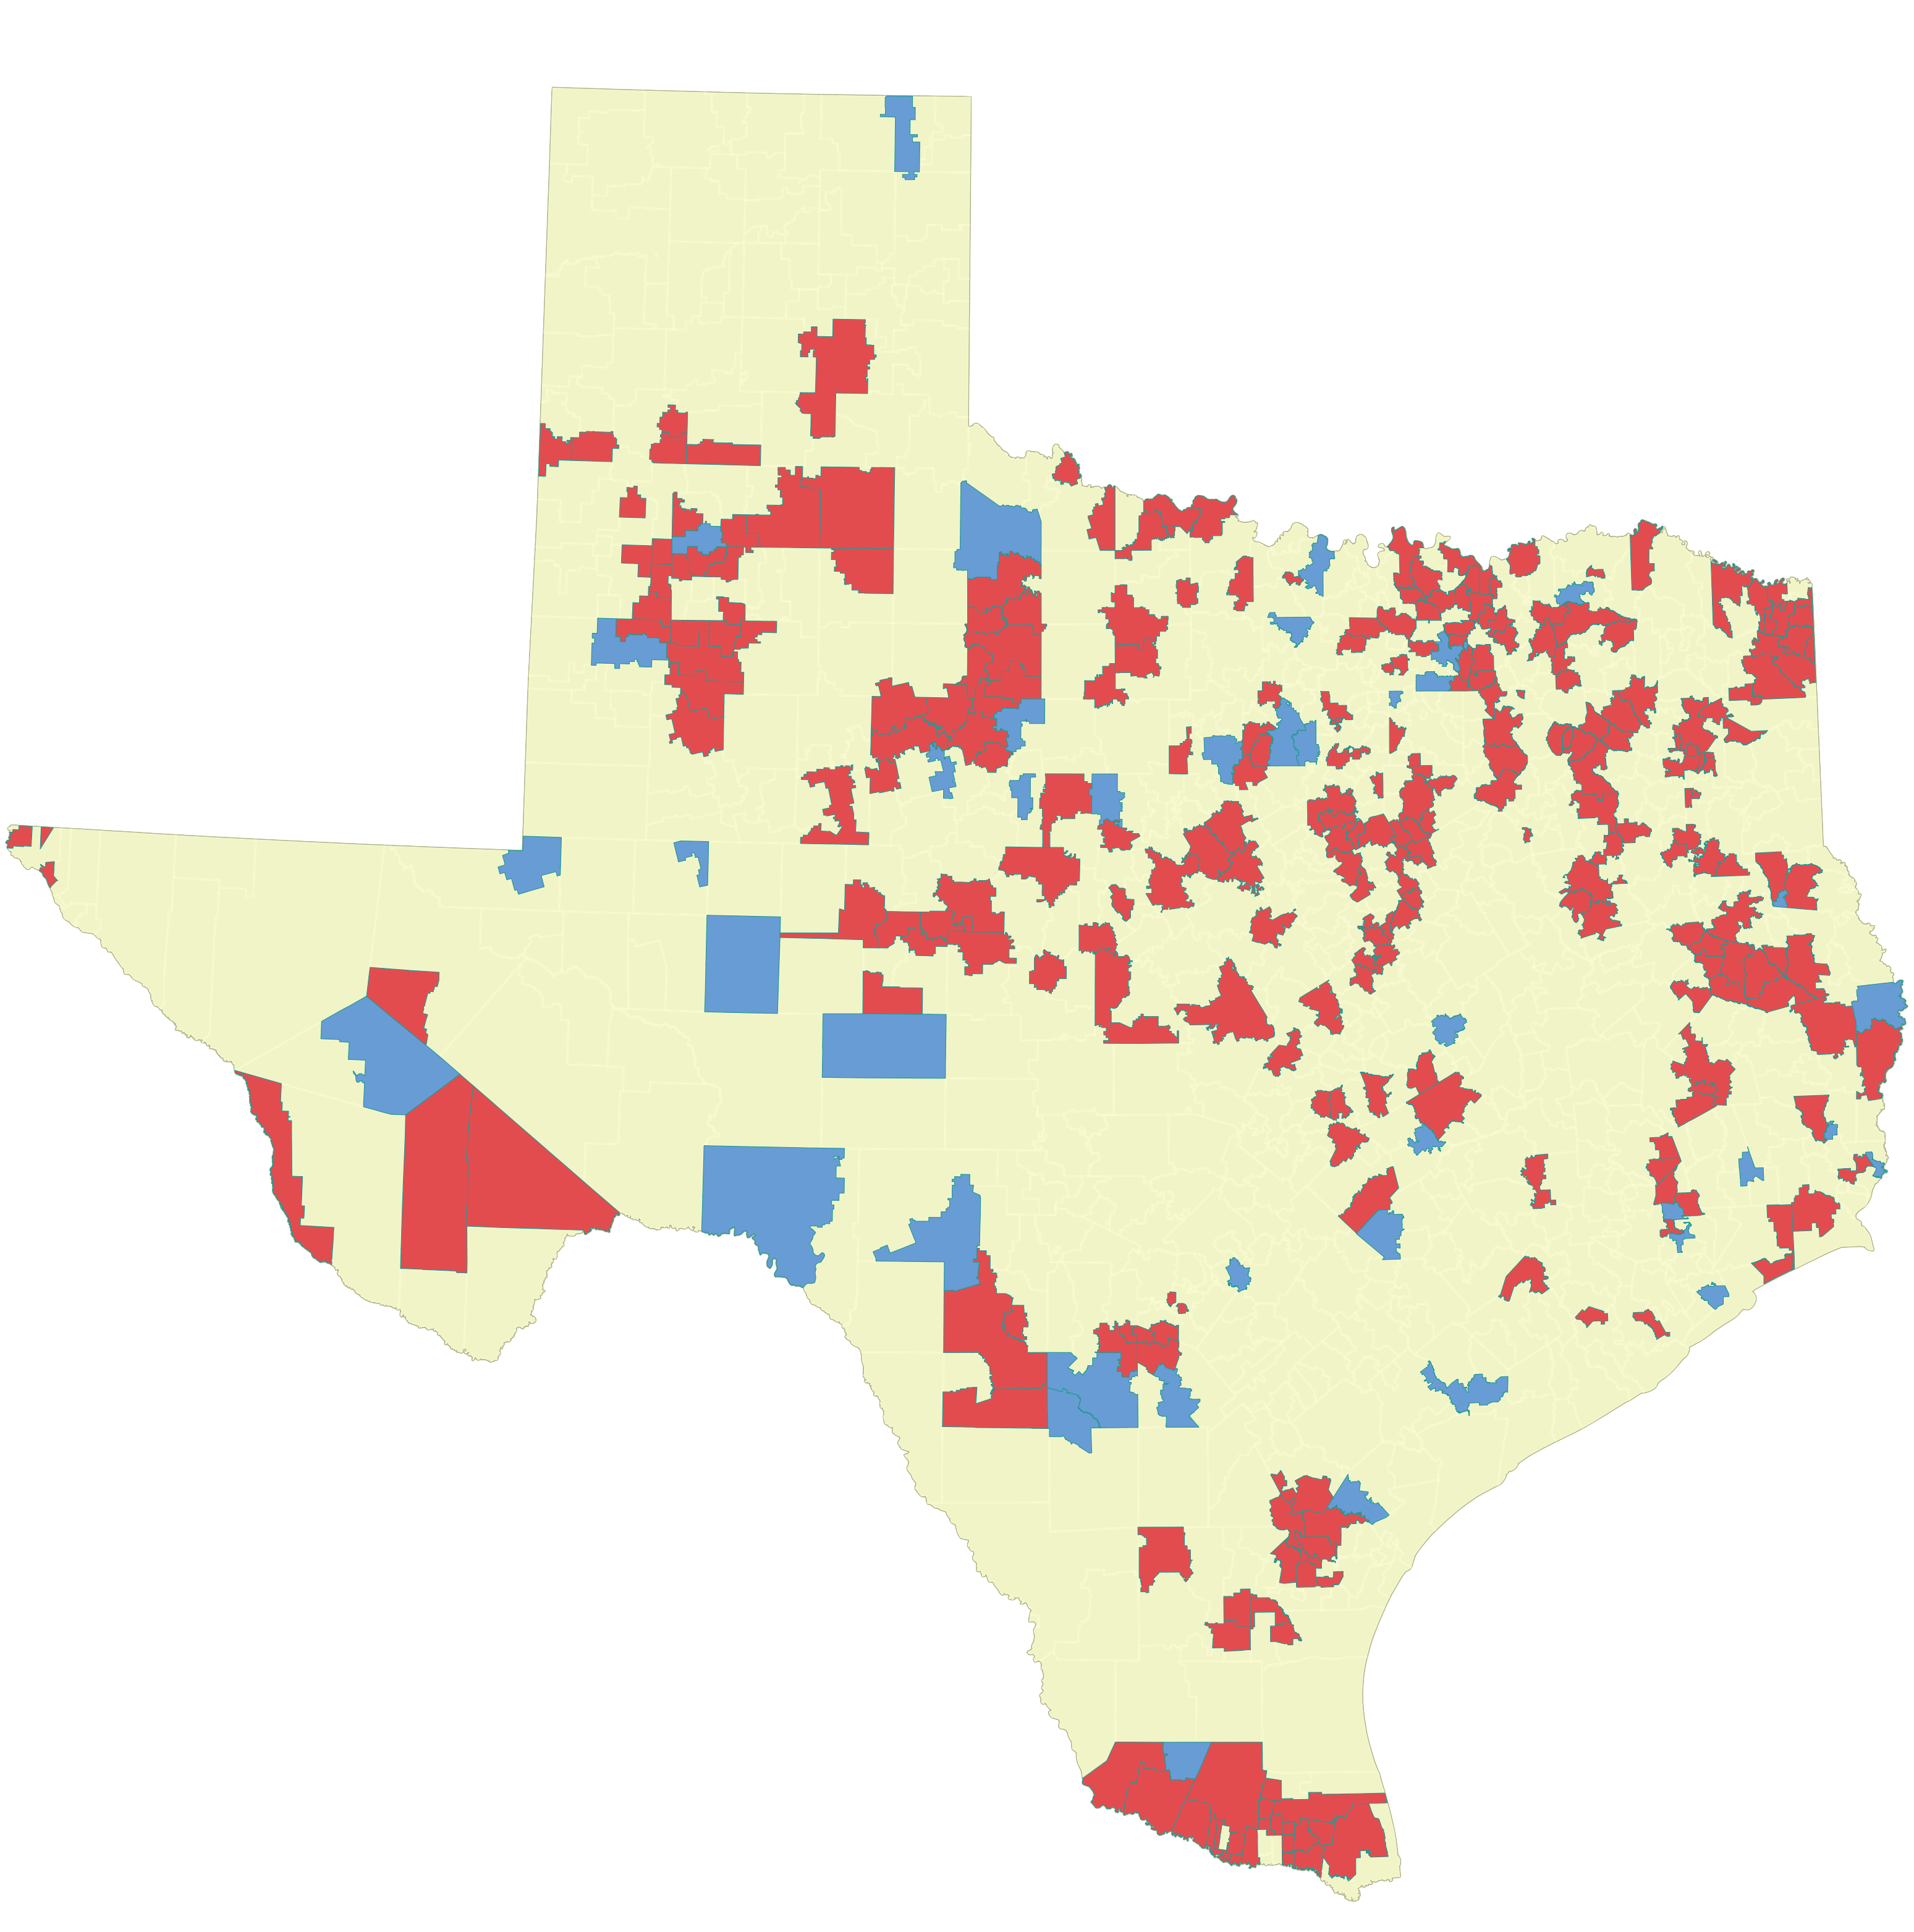
\includegraphics[height=14cm]{images/Texas2.png}\\\vskip.5cm}
  % 
\includegraphics[height=1cm]{images/UT Logos/LBJ/Text_SmallCenter.png}\\\vskip.5cm}
  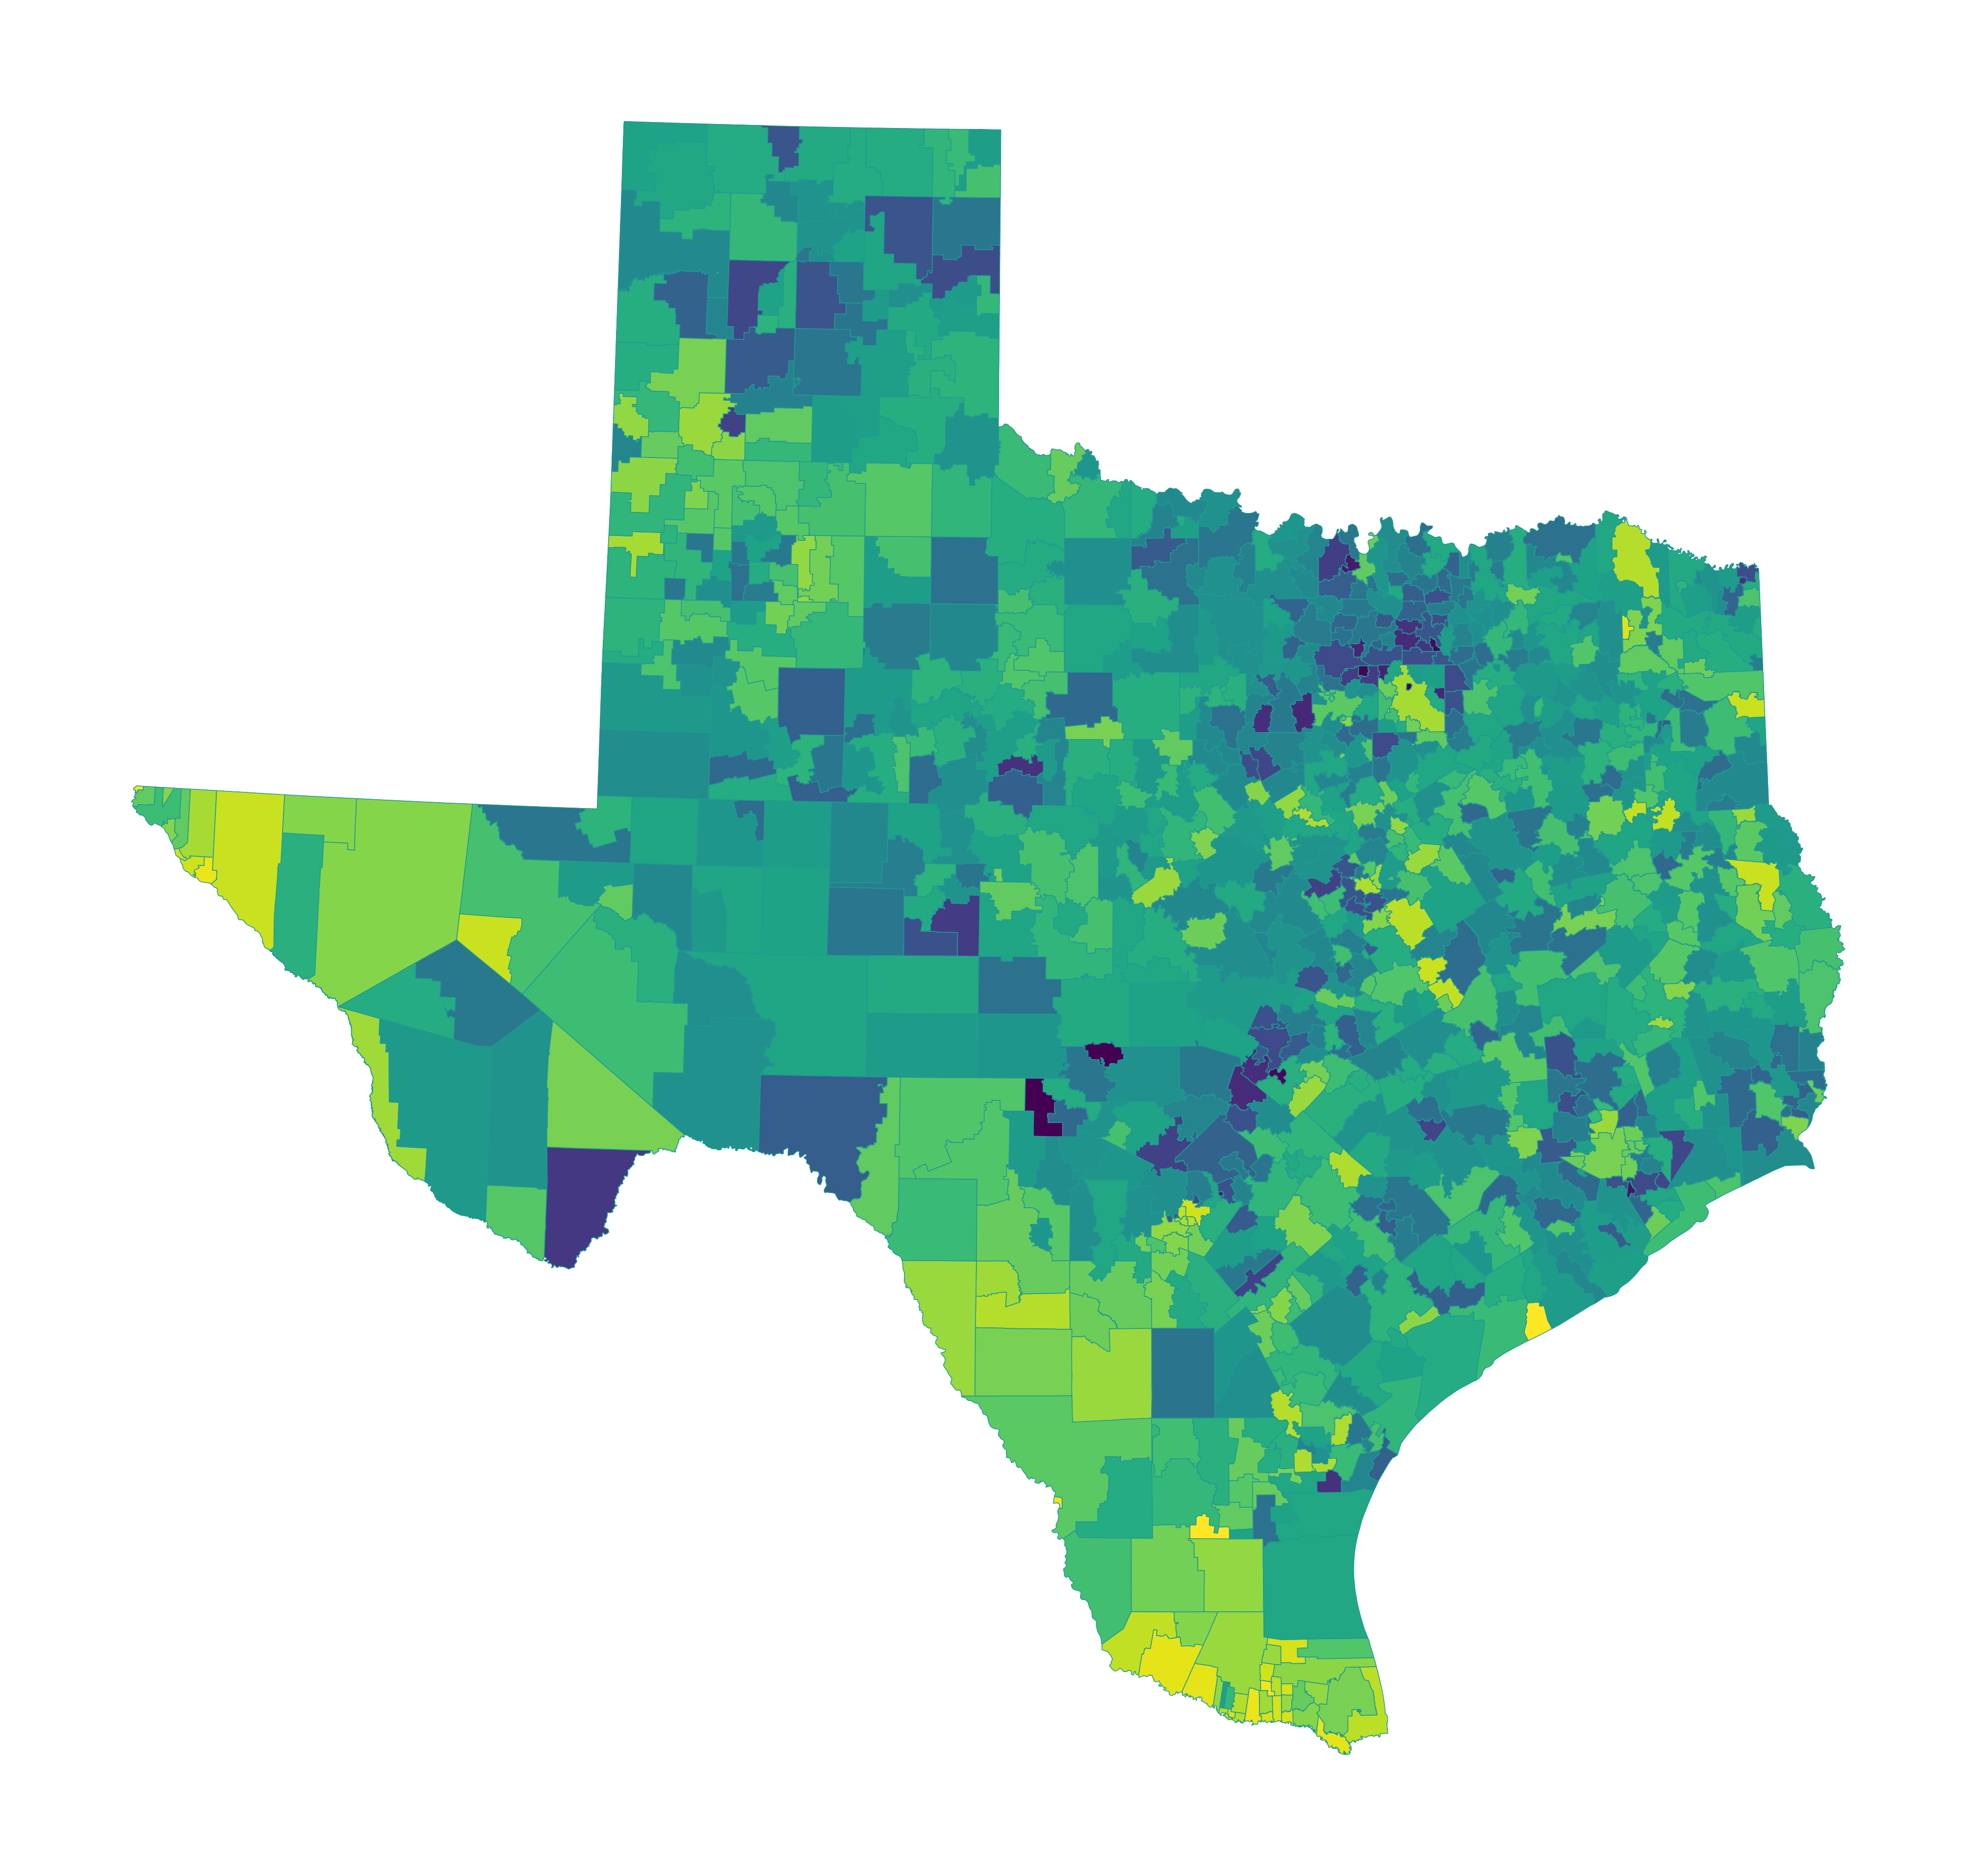
\includegraphics[height=14cm]{images/Texas.png}\\\vskip.5cm}
  % 
\includegraphics[height=5cm]{images/UT Logos/UTAustin/UT_Seal.png}\\\vskip.5cm}


%Set Header and Footers For Regular Text Pages
\setlength\headheight{26pt}
\usepackage{fancyhdr}
\usepackage{lastpage}
\pagestyle{fancy}
\fancyhf{}
\fancyhead[LE,RO]{Worthington}
% \fancyhead[RE,LO]{Solutions for America's Children in Poverty}
\fancyhead[RE,LO]{
\includegraphics[height=.4cm]{images/UT Logos/LBJ/Text_Big.png}}
\fancyhead[CE,CO]{Solutions for America's Children in Poverty}
\fancyfoot[CE,CO]{}
\fancyfoot[LE,RO]{\thepage \hspace{1pt} of \pageref{LastPage}}

%Define Style for Landscape Map Attachments
\renewcommand{\listfigurename}{List of Maps and Figures}
\renewcommand{\listtablename}{Tables}
\fancypagestyle{lscapedplain}{%
  \setlength{\footskip}{30pt}
  \renewcommand{\headrulewidth}{0pt}
  \fancyhf{}
  \fancyfoot{%
    \tikz[remember picture,overlay]
      \node[outer sep=1cm,above,rotate=90] at (current page.east) {\thepage};}
}

%Load Other Packages
\usepackage{calc}  
\usepackage{enumitem}
\usepackage{setspace}
\usepackage{epigraph}
\usepackage{geometry}
\usepackage{marginnote}
\usepackage{sectsty}
\usepackage{booktabs}
\usepackage{wrapfig}
\usepackage{scrextend}
\usepackage{pdfpages}
\usepackage{pdflscape}

%For Fancy Header and Footer Lines
\renewcommand{\headrulewidth}{.5pt}
%\renewcommand{\footrulewidth}{1pt}

%Adjust Figure Position, Width, & Wrap
\usepackage{float}
\let\origfigure\figure
\let\endorigfigure\endfigure
\renewenvironment{figure}[1][2] {
    \expandafter\origfigure\expandafter[H]
} {
    \endorigfigure
}
\usepackage{graphicx}
\setkeys{Gin}{width=.9\linewidth}

%Section Paragraph Formatting 
%\usepackage[table]{xcolor} % If not using pdfpages, then reinvoke this package
\definecolor{gray}{rgb}{.302,.302,.302}
\definecolor{blue}{rgb}{.365, .647, .855}
\definecolor{orange}{rgb}{.98,.643,.227}
\definecolor{green}{rgb}{.376,.741,.408}
\definecolor{pink}{rgb}{.945,.486,.69}
\definecolor{brown}{rgb}{.698,.569,.184}
\definecolor{purple}{rgb}{.698,.463,.698}
\definecolor{yellow}{rgb}{.871,.812,.247}
\definecolor{red}{rgb}{.945,.345,.329}
\definecolor{textgray1}{rgb}{.40,.431,.459} % HEX #282b2d
\definecolor{textgray2}{rgb}{.38,.38,.38} % HEX #262626
\definecolor{textgray3}{rgb}{.282,.282,.282} % HEX #1c1c1c
\definecolor{gray75}{gray}{0.75}
\definecolor{utorange}{rgb}{.749,.341,0} %HEX #bf5700
\definecolor{utgray}{rgb}{.20,.247,.282} %HEX #333f48
\definecolor{utgray75}{rgb}{.40,.431,.459} %HEX #666e75
\definecolor{utblue}{rgb}{0,.373,.525} %HEX #005f86
\definecolor{utblue75}{rgb}{.235,.529,.639}
\definecolor{utblue50}{rgb}{.,.529,.639}
\definecolor{utred}{rgb}{.78, .071, .192}
\definecolor{utgreen}{rgb}{	.263, .412, .357}
\definecolor{googletext2}{rgb}{.259,.259,.259}
\color{utgray75}
\color{black}
\usepackage{titlesec}
\newcommand{\hsp}{\hspace{15pt}}
%\renewcommand{\thesection}{}
\titleformat{\chapter}[hang]{\normalfont\huge\bfseries\singlespacing\color{utgray}}{\color{utorange}\thechapter\hsp\textcolor{gray75}{|}\hsp}{0pt}{\huge\bfseries}
\titleformat{\section}{\singlespacing\normalfont\LARGE\bfseries\color{utblue}}{}{0em}{}
\titleformat{\subsection}{\singlespacing\normalfont\large\bfseries}{\thesubsection}{1em}{}
\titleformat{\subsubsection}{\singlespacing\normalfont\normalsize\bfseries}{\thesubsubsection}{1em}{}
%\addtolength{\leftskip}{\widthof{\normalfont\bfseries\makebox[1.9em]{}}}% Indent text
\widowpenalty=1000
\clubpenalty=1000

% %Figures, Tables, & Maps List
% \renewcommand{\listfigurename}{List of plots}
% \renewcommand{\listtablename}{Tables}